\documentclass[12]{article}
\usepackage{graphicx}
\usepackage{color}
\usepackage{algorithmic}
\begin{document}

\title{\textbf{
\includegraphics[scale=0.5]{42.png}
\textcolor{red}{Universitatea din Craiova \\Facultatea de Automatic\u{a},Calculatoare \c{s}i Electronic\u{a}}}}
\date{\textbf{04 June 2018}}
\maketitle
\begin{center}
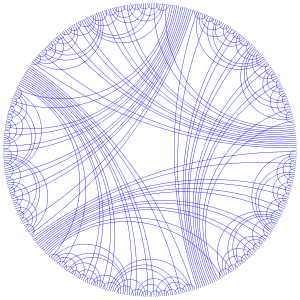
\includegraphics[scale=0.7]{cover_graph.png}
\end{center}
\textbf{Project : Algorithm Design} \\
\textbf{Title: Minimum Length Path}\\
\textbf{Teachers: Becheru Alex \& B\u{a}dic\u{a} Costin}\\
\textbf{Student: Amzuloiu Andrei-Ciprian} \\
\textbf{Section : Calculatoare Rom\^{a}n\u{a}\\ Year I\\ Group: CR 1.1}
\newpage
\tableofcontents

\newpage
\section{Problem Statement}

\textcolor{white}{}
\subsection{Title}
         \textcolor{blue}    {Minimum Length Path.}

\subsection{Description}
\textcolor{white}{}


My assignment requires the implementation of two different algorithms to determine the minimum path between two vertexes in weighted directed graphs.

To done that I implemented the Bellman Ford algorithm and the Dijkstra’s algorithm in C.

\newpage

\section{Pseudocode}

\subsection{convert\_mat\_array($$ INT coordinates_1, INT coordinates\_2, INT maximum\_size$)}
\begin{algorithmic}[1]
\STATE $return \ coordinate\_1 * maximum\_size + coordinates\_1$
\end{algorithmic}

\subsection{random\_graph(struct graph* graph)}
\begin{algorithmic}[1]

    \STATE $INT \ iterator_1$
    \STATE $INT \ iterator_2$
    \STATE $INT \ flag$
    
    \STATE $graph -> no\_elems = rand()$
    \STATE $graph -> \ no\_edges = 0$

    \STATE $graph -> \ ad\_matrix = calloc(graph -> no\_elems \ * \ graph \-> no\_elems, \  sizeof(int))$

    \FOR{ $iterator_1 = 0 \ \TO \ graph -> no\_elems $}
        \FOR{ $iterator_2 = 0 \ \TO \ graph -> no\_elems$}
            
            \IF{ $(iterator_1 == iterator_2)$ }
            \STATE $continue$
            \ENDIF
            \STATE $flag = rand()$
            
            \IF{ $(flag)$ }
                \STATE $graph -> no\_edges++$

                
                \IF{ $graph -> ad\_matrix[convert\_mat\_array(iterator_2, \  iterator_1, \  graph -> \ no\_elems)] == 0)$ }
                    \STATE $graph -> ad\_matrix[convert\_mat\_array(iterator_1, iterator_2, graph -> no\_elems)] = rand() $
                \ENDIF
            \ENDIF 
        \ENDFOR
    \ENDFOR

\end{algorithmic}


\subsection{create\_edges(struct graph* graph)}
\begin{algorithmic}[1]

    \STATE $INT \ iterator $
	\STATE $INT \ iterator\_edge = 0 $

	
	\STATE $graph -> \  edge = (struct edge\*) malloc( graph   -> \ no_edges \* sizeof( struct edge ) )$

	\FOR{ $iterator = 0 \  \TO  \  graph -> \ no\_elems \* graph -> \ no\_elems $}
		\IF{ $(graph ->\ ad\_matrix[iterator] != 0)$}
		\STATE	$graph ->\ edge[iterator\_edge].source = iterator / graph ->\ no\_elems$
		\STATE	$graph ->\ edge[iterator\_edge].destination = iterator \% graph -> no\_elems$
		\STATE	$graph ->\ edge[iterator\_edge].weight = graph -> ad\_matrix[iterator]$
		\STATE	$iterator\_edge++$
		\ENDIF
	\ENDFOR

\end{algorithmic}

\subsection{negative\_cycle\_check(struct graph graph, INT dist[ ])}
\begin{algorithmic}[1]

    \STATE $INT \ iterator $
	\STATE $INT \ source $
	\STATE $INT \ destination $
	\STATE $INT \ weight $

	\FOR{ $iterator = 0 \  \TO \  graph.no_edges $ }
        \STATE  $source = graph.edge[iterator].source;$
        \STATE $destination = graph.edge[iterator].destination$
        \STATE $weight = graph.edge[iterator].weight$

        \IF {$( dist[source] != INFINITY\ \&\&\ dist[source] + weight < dist[destination] )$}
            \STATE $print("Graph\ contains\ negative\ weight\ cycle\!\ Bellman\ Ford\ algorithm\ is\ unavailable\.")$
        	\STATE $return\ 1$
        \ENDIF
    \ENDFOR

    \STATE  $ return \  0 $

\end{algorithmic}

\subsection{init\_dijkstra (struct graph graph, INT value\_mat[ ], INT distance[ ], INT pred[ ], int start\_node)}
\begin{algorithmic}[1]
    \STATE $INT\ iterator_1$
	\STATE $INT\ iterator_2$

	\FOR{ $iterator\_1 = 0 \  \TO \ graph.no\_elems$ }
        \FOR{ $iterator_2 = 0 \ \TO \ graph.no_elems$ }
            \IF($ graph.ad\_matrix[convert\_mat\_array(iterator_1, iterator_2, graph.no\_elems)] == 0 $)
                \STATE $value\_mat[convert\_mat\_array(iterator_1, iterator_2, graph.no\_elems)] = INFINITY$
             \ELSE 
                \STATE $value\_mat[convert\_mat\_array(iterator_1, iterator_2, graph.no\_elems)] = graph.ad\_matrix[convert\_mat\_array(iterator\_1, iterator\_2, graph.no\_elems)]$
            \ENDIF
        \ENDFOR
    \ENDFOR
    
    FOR{ $iterator_1 = 0 \ \TO \ graph.no\_elems$}{
        \STATE $distance[iterator_1] = value\_mat[convert\_mat\_array(start\_node, iterator_1, graph.no\_elems)]$
        \STATE $pred[iterator_1] = start\_node$
    }
\end{algorithmic}


\subsection{print\_results\_dijkstra( INT dist[ ], INT path[ ][ ], INT no\_elems )}
\begin{algorithmic}[1]
    \STATE $INT\ iterator$

	\IF{$( final\_node != start\_node )$}
        \IF{$( distance[final\_node] < INFINITY )$}
           \STATE $print("Distance\ between\ \% d\ and\ \%d : \%d", start\_node,\ final\_node, distance[final\_node])$
          \STATE  $print("Path: \%d ", final\_node)$
        
           \STATE $iterator = final\_node$

            \WHILE{$(iterator != start\_node)$}
              \STATE $iterator = pred[iterator]$
              \STATE $print("<- \%d ", iterator)$
             \ENDWHILE
            
        \ELSE
            print("No valid path between the two vertexes.");
        \ENDIF

    \ELSE 
        $print("Distance between \%d and \%d : \%d", start\_node, final\_node, distance[final\_node])$
        $print("Path: \%d", start\_node)$
    \ENDIF
\end{algorithmic}

\subsection{init\_bellman\_ford( int dist[ ], INT path[ ][ ], INT no\_elems )}
\begin{algorithmic}[1]
\STATE $INT\ iterator$

\FOR{ $iterator = 0 \ \TO \ no\_elems$}
        \STATE $dist[iterator] = INFINITY$
    \ENDFOR

    \FOR{$iterator = 0 \ \TO \ no\_elems$}
        \STATE $path[iterator][0] = 0$
    \ENDFOR
\end{algorithmic}

\subsection{print\_results\_bellman\_ford( INT dist[ ], INT path[ ][ ], INT no\_elems )}
\begin{algorithmic}[1]
    \STATE $INT\ iterator$

	\IF{ dist[dest] == INFINITY }
        \STATE $print("No\ valid\ path\ between\ the\ two\ vertexes.")$
     \ELSE 
        \STATE $print("Distance\ between \%d\ and \%d\ : \%d",\ src,\ dest,\ dist[dest])$
        \STATE $print("Path: \%d ",\ dest)$
        \FOR{ $iterator = path[dest][0] \TO 0$ }
            \STATE $print("<- \%d ",\ path[dest][iterator])$
            \ENDFOR
        
    \ENDIF
\end{algorithmic}

\subsection{dijkstra( struct graph graph, INT start\_node, INT final\_node)}
\begin{algorithmic}[1]
    \STATE $INT\ *value\_mat = (int*) malloc(graph.no\_elems * graph.no\_elems * sizeof(int))$
    \STATE $INT\ *distance = (int*) malloc(graph.no\_elems * sizeof(int))$
    \STATE $INT\ *pred = (int*) malloc(graph.no\_elems * sizeof(int))$
    \STATE $INT\ *visited = (int*) calloc(graph.no\_elems, sizeof(int))$
    \STATE $INT\ count$
    \STATE $INT\ minimum\_distance$
    \STATE $INT\ next\_node$
    \STATE $INT\ iterator_1$
    \STATE $INT\ iterator_2$
    
    \STATE $init\_dijkstra(graph, value\_mat, distance, pred, start\_node)$
    
    \STATE $distance[start\_node] = 0$
    \STATE $visited[start\_node] = 1$
    \STATE $count = 1$
    
    \WHILE{$(count < graph.no\_elems - 1 )$}
        \STATE $minimum\_distance = INFINITY$
        
        \FOR{ $iterator_1 = 0\ \TO \ graph.no\_elems$ }
            \IF{$( distance[iterator_1] < minimum\_distance && !visited[iterator_1] )$}
                \STATE $minimum\_distance = distance[iterator_1]$
                \STATE $next\_node = iterator_1$
            \ENDIF
        \ENDFOR
                    
        \STATE $visited[next\_node] = 1$
        \FOR{ $iterator_1 = 0 \ \TO \ graph.no\_elems$}
            \IF{$( !visited[iterator_1] )$}
                \IF{$( minimum\_distance + value\_mat[convert\_mat\_array(next\_node, iterator_1, graph.no\_elems)] < distance[iterator_1] )$}
                    \STATE $distance[iterator_1] = minimum\_distance +  value\_mat[convert\_mat\_array(next\_node, iterator_1, graph.no\_elems)]$
                    \STATE $pred[iterator_1] = next\_node$
                \ENDIF
            \ENDIF
        \ENDFOR

        \STATE $count++$
    \ENDWHILE

    \STATE $print\_results\_dijkstra(start\_node, final\_node, distance, pred)$
    \STATE $free(value_mat)$
    \STATE $free(distance)$
    \STATE $free(pred)$
    \STATE $free(visited)$

\end{algorithmic}

\subsection{bellman\_ford( struct graph graph, INT start\_node, INT final\_node)}
\begin{algorithmic}[1]

    \STATE $INT \ *dist = (int*) malloc(graph.no\_elems * sizeof(int))$
    \STATE $INT \ iterator_1$
    \STATE $INT \ iterator_2$
    \STATE $INT \ iterator_3$
    \STATE $INT \ weight$
    \STATE $INT \ source$
    \STATE $INT \ destination$
    \STATE $INT \ **path = (int**) malloc(graph.no_elems * sizeof(int*))$
    \FOR {$iterator_1 = 0 \ \TO \ iterator_1 < graph.no_elems$}
        \STATE $path[iterator_1] = (int*) malloc(graph.no\_elems * sizeof(int))$
    \ENDFOR

    \STATE $create_edges(&graph)$

    \STATE $init_bellman_ford( dist, path, graph.no\_elems )$
    \STATE $dist[start\_node] = 0$

    \FOR{$iterator_1 = 1 \ \TO \  graph.no\_elems - 1 $}
        \FOR{$iterator_2 = 0 \ \TO \ graph.no\_edges$}
            \STATE $source = graph.edge[iterator_2].source$
            \STATE $destination = graph.edge[iterator_2].destination$
            \STATE $weight = graph.edge[iterator_2].weight$

            \IF{$( dist[source] != INFINITY && dist[source] + weight < dist[destination] )$}
                \STATE $dist[destination] = dist[source] + weight$

                \STATE $path[destination][0] = path[source][0] + 1$
                \FOR{$iterator_3 = 1 \ \TO \  path[destination][0]$}
                    \STATE $path[destination][iterator_3] = path[source][iterator_3]$
                \ENDFOR
                \STATE $path[destination][ path[destination][0] ] = source$
            \ENDIF
        \ENDFOR
    \ENDFOR
 
    \IF{ $(!negative\_cycle\_check(graph, dist) )$}
        \STATE $print\_results\_bellman\_ford(start\_node, final\_node, dist, path)$
    \ENDIF
    
    \STATE $free(dist)$
    \FOR{$ iterator_1 = 0 \ \TO \ graph.no\_elems$}
        \STATE $free(path[iterator_1])$
    \ENDFOR
    \STATE $free(path)$
    \STATE $free(graph.edge)$

\end{algorithmic}

\subsection{print\_ad\_mat( struct graph graph )}
\begin{algorithmic}[1]

	\STATE $FILE \  *f\_write$
    \STATE $INT iterator$

    \STATE $f\_write = open("graph.txt", "w")$
    \STATE $print(f\_write, "Number\ of\ vertexes: \%d Adjacency\ matrix\ with\ cost\ on\ each\ edge: NEW\ LINE", graph.no\_elems)$
    \FOR{$ iterator = 0 \ \TO \ graph.no\_elems * graph.no\_elems $}
        \STATE $print(f\_write, "\%d ", graph.ad\_matrix[iterator])$
        \IF{$(iterator \% graph.no\_elems == graph.no\_elems - 1)$}
            \STATE $print(f_write, NEW LINE)$
        \ENDIF
    \ENDFOR

    \STATE $close(f\_write)$
\end{algorithmic}

\subsection{read\_input( INT var_1, INT var_2 )}
\begin{algorithmic}[1]
    \STATE $FILE *f\_read$

	\STATE $f\_read = open("input.txt", "r")$
	\STATE $scan(f\_read, "\%d\%d", var_1, var_2)$

	\STATE $close(f\_read)$
\end{algorithmic}

\newpage
\section{Application Design}
\subsection{Main}
\textbf{}

This module has the user interaction part and some functions calls ( random\_graph(), print\_ad\_mat(), read\_input(), bellman\_ford() and dijkstra() functions ).

I used the random\_graph() function to generate a random weighted directed graph. The graph is stored in $graph$, a structure variable. After that, the adjacency matrix with cost edges is printed in $graph.txt$ using the print\_ad\_mat() function, because it's easier for user to check it in file then checking from the console screen.
I used the $keep\_open$ variable to put a pause in the running to allow the user to check the graph in file and choose the source vertex and destination vertex. The source and destination vertex are written by the user in the &input.txt& file. 

After all, I called the  bellman\_ford() function and the dijkstra() function and put another pause in the console screen to allow the user to check the results.

\subsection{dijkstra() function}
\textbf{}

Dijkstra algorithm is also called single source shortest path algorithm. It is based on greedy technique. The algorithm maintains a list visited[ ] of vertices, whose shortest distance from the source is already known.
 If visited[1], equals 1, then the shortest distance of vertex i is already known. Initially, visited[i] is marked as, for source vertex.
 At each step, we mark visited[v] as 1. Vertex v is a vertex at shortest distance from the source vertex. At each step of the algorithm, shortest distance of each vertex is stored in an array distance[ ].
 
 The steps for Dijkstra algorithm is:
 
 1. Create cost matrix (value\_mat[ ], in our case) from adjacency matrix (graph.ad\_matrix). value\_mat[i, j, graph.no\_elems)] is the cost of going from vertex i to vertex j. If there is no edge between vertices i and j then value\_mat[i, j, graph.no\_elems)] is infinity. 
 
 I used array instead of matrices. To convert the coordinates of a matrix in array position I used the function convert\_mat\_array(). It returns the converted array position. 
 
 2. Array visited[ ] is initialized to zero. To done that I allocated memory using function calloc.
 
 3. If the vertex 0 is the source vertex then visited[0] is marked as 1.
 
 4. Create the distance matrix, by storing the cost of vertices from vertex no. 0 to graph.no\_elems - 1 from the source vertex 0. Initially, distance of source vertex is taken as 0. i.e. distance[0] = 0.
 
 I done the step 1, 3 and 4 in the function init\_dijkstra().
 
 
 5. Iterate from 1 to graph.no\_elems
 
– Choose a vertex next\_node, such that distance[next\_node] is minimum and visited[next\_node] is 0. - Mark visited[next\_node] as 1.

– Recalculate the shortest distance of remaining vertices from the source.

– Only, the vertices not marked as 1 in array visited[ ] should be considered for recalculation of distance.
   
   At the end I called the function print\_results\_dijkstra() to print the distance and path in the console scree. I used the $time.h$ library to find the execution time.
   
 
 The program contains two loops each of which has a complexity of O(n). n is number of vertices. So the complexity of algorithm is O($n^2$).

\subsection{bellman\_ford() function}
\textbf{}
Dijkstra and Bellman-Ford Algorithms used to find out single source shortest paths. i.e. there is a source node, from that node we have to find shortest distance to every other node. Dijkstra algorithm fails when graph has negative weight cycle. But Bellman-Ford Algorithm won’t fail even, the graph has negative edge cycle. (using negative\_cycle\_check() function in our case) If there any negative edge cycle it will detect and say there is negative edge cycle. If not it will give answer to given problem.

Bellman-Ford Algorithm will work on logic that, if graph has n nodes, then shortest path never contain more than n - 1 edges. This is exactly what Bellman-Ford do. It is enough to check each edge (graph.no\_edges - 1) times to find shortest path. But to find whether there is negative cycle or not we again do one more relaxation. If we get less distance in $n^t^h$ relaxation we can say that there is negative edge cycle. Reason for this is negative value added and distance get reduced.

Following are the detailed steps.


1) This step initializes distances from source to all vertices as infinite and distance to source itself as 0. Create an array dist[] of size graph.no\_elems with all values as infinite except dist[start\_node] where start\_node is source vertex. This step is included in the init\_bellman\_ford() function. This algorithms works with edges so I used the create\_edges() function to find all edges (with source, destination and weight) from adjacency matrix.

2) This step calculates shortest distances. Do following ( graph.no\_edges - 1 ) times where graph.no\_edges is the number of vertices in given graph. If a better way is found the distance is added in the distance array and the path in the path matrix (path[ ][ ]) which is a matrix where all paths with minimum distances are stored.

3) This step reports if there is a negative weight cycle in graph. To done that I used the negative\_cycle\_check() function.

The idea of step 3 is, step 2 guarantees shortest distances if graph does not contain negative weight cycle. If we iterate through all edges one more time and get a shorter path for any vertex, then there is a negative weight cycle.

The time complexity is (v-1) (E) O(1) = O(VE).

\subsection{random\_graph() function}
\textbf{}

The graph is a non-trivial concept, so I used a generator to generate a graph with big number of elements (up to 500). The function uses the rand() function to generate the number of nodes. After that, each element of the matrix is iterated. When flag == 1 there will be an edge, else the position in ad\_matrix will be 0. The rand() is used again to change the value of flag (1 or 0) and to give a value to each edge of the graph (a adjiancy matrix position). 

\subsection{Input//Output}
\textbf{}

The generated graph is printed in  file graph.txt. The only input of the program are the two vertexes (source and destination) from the input.txt. After the user check the graph, he can choose two vertexes to find the minimum distance and path of them. 

The results (distance, path and time execution of each algorithm) will be printed in the console screen. 

\subsection{Modules}
\textbf{}

I used two header files.


1) $algorithms.h$, a C library implementation for Dijkstra algorithm and Bellman Ford algorithm. This library has the following functions:

- \textbf{void dijkstra( struct graph graph, int start\_node, int final\_node );}

This function is used to find the minimum path between two vertexes and print them in console screen using the Dijkstra algorithm.

Parameters:

        graph - A structure variable that contains the details about the graph that will be used.
        
        start\_node - The source vertex.
        
        final\_node - The destination vertex.
        
- \textbf{void bellman\_ford( struct graph graph, int start\_node, int final\_node );}

This function is used to find the minimum path between two vertexes and print them in console screen using the Bellman Ford algorithm.

Parameters:

    graph - A structure variable that contains the details about the graph that will be used.
    
        start\_node - The source vertex.
        
        final\_node - The destination vertex.
        
2) $tools.h$, a  C library implementation for some functions used in algorithms or used for input/output. This library has the following functions:

- \textbf{int convert\_mat\_array( int coord\_1, int coord\_2, int max\_size );}

This function converts the coordinates of a matrix in array position and return the value of that position.

Parameters:

    coord\_1 - The column coordinate of a matrix.
 
    coord\_2 - The row coordinate of a matrix.

    max\_size - The size of a row/column.

- \textbf{void create\_edges( struct graph* graph );}

This function use the ad\_matrix to create an array with all edges of the graph. This function is used in the Bellman Ford algorithm because it works with the edges of the graph.

    Parameters:
    
    *graph - The graph that we use in our algorithms.
    
- \textbf{void random\_graph( struct graph* graph );}

This function is used to generate a random graph.

    Parameters:
    
    *graph - A struct variable that we use to generate the graph.

- \textbf{void print\_ad\_mat( struct graph graph );}

This function is used to print the adjacency matrix in graph.txt.

    Parameters:
    
    graph - A structure variable that contains the details about the graph that will be used.

- \textbf{void read\_input( int* var\_1, int* var\_2 );}

This function is used to read the source vertex and the destination vertex from input.txt.

Parameters:

        *var\_1 - The source vertex.
        
		*var\_2 - The destination vertex.
		
- \textbf{void init\_dijkstra( struct graph graph, int* value\_mat, int* distance, int* pred, int start\_node );}

This function is used to initialize the value\_mat, distace and pred arrays for the Dijkstra algorithm.


Parameters:
        
        graph - A structure variable that contains the details about the graph that will be used.
        
        *value\_mat - A copy of *ad\_matrix modified for dijkstra algorithm.
        
	    *distance - An array used to store the distance between source vertex and any other vertex in graph.
	    
    	*pred - An array used to store the predecessor of each node.
    	
- \textbf{void print\_results\_dijkstra( int start\_node, int final\_node, int* distance, int* pred );}

This function is used to print the minimum distance and path between two vertexes after the implementation of the Dijkstra algorithm.

Parameters:

start\_node - The source vertex.

 final\_node - The destination vertex.
 
	*distance - An array used to store the distance between the source vertex and any other vertex.
	
*pred - An array used to store the predecessor of each node.
    

- \textbf{void init\_bellman\_ford( int* dist, int** path, int no\_elems );}

This function is used to initialize the dist array and the path matrix for the Bellman Ford algorithm.

Parameters: 

		*dist - An array used to store the distance between the source vertex and any other vertexes.
		
		**path - A matrix used to store the path between source vertex and any other vertexes.
		
		no\_elems - The number of vertexes.

- \textbf{void print\_results\_bellman\_ford( int src, int dest, int* dist, int** path );}

This function is used to print the minimum distance and path between two vertexes after the implementation of the Bellman Ford algorithm.

Parameters:

src - The source vertex.

 dest - The destination vertex.
 
 *dist - An array used to store the distance between the source vertex and any other vertexes.
 
 **path - A matrix used to store the path between the source vertex and any other vertex of the graph.
		

- \textbf{int negative\_cycle\_check( struct graph graph, int* dist );}


This function is used to check if the graph has negative cycles. I used this function in the Bellman Ford algorithm.

Parameters: 

graph - A structure variable that contains the details about the graph that will be used.

*dist - An array used to store the distance between the source vertex and any other vertexes.		

Also, in the tools.h library I declared two structures. First is the structure $edge$ which contain details about an edge (source vertex, destination vertex, the weight of the edge). The second is the structure $graph$ which contain details about the used grah (number of nodes, number of edges, adjacency matrix and an array of all edges stored in graph).

\subsection{Experiments}
\textbf{}

I ran the program few times to see the difference between the execution time of the two algorithms.

For a random generated graph with 102 vertexes:

\begin{center}
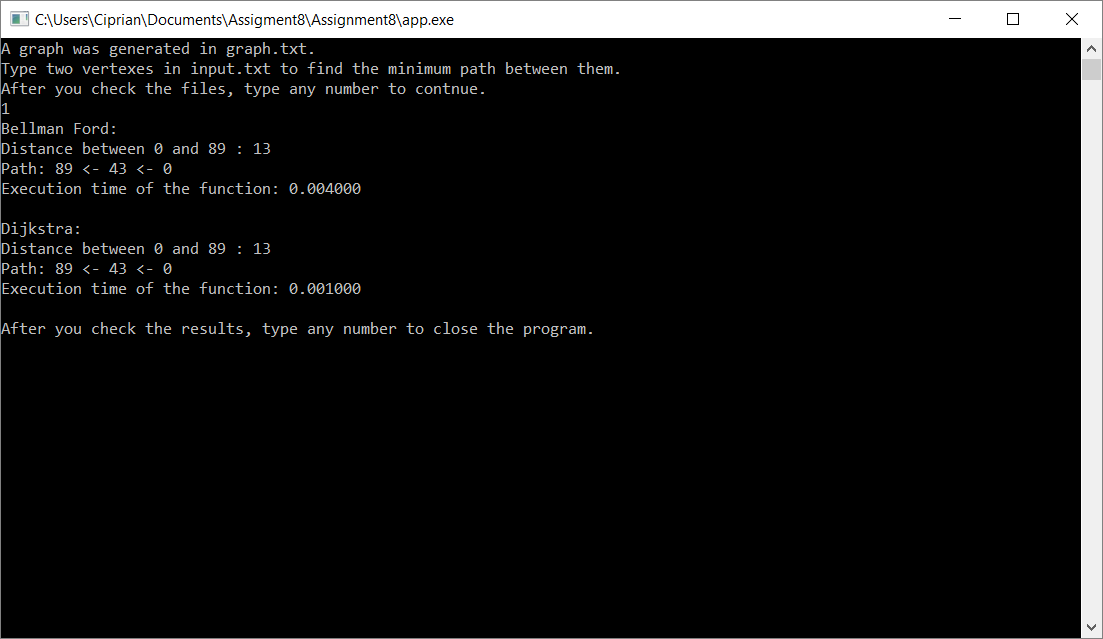
\includegraphics[scale=0.6]{102.png}
\end{center}

For a random generated graph with 217 vertexes:

\begin{center}
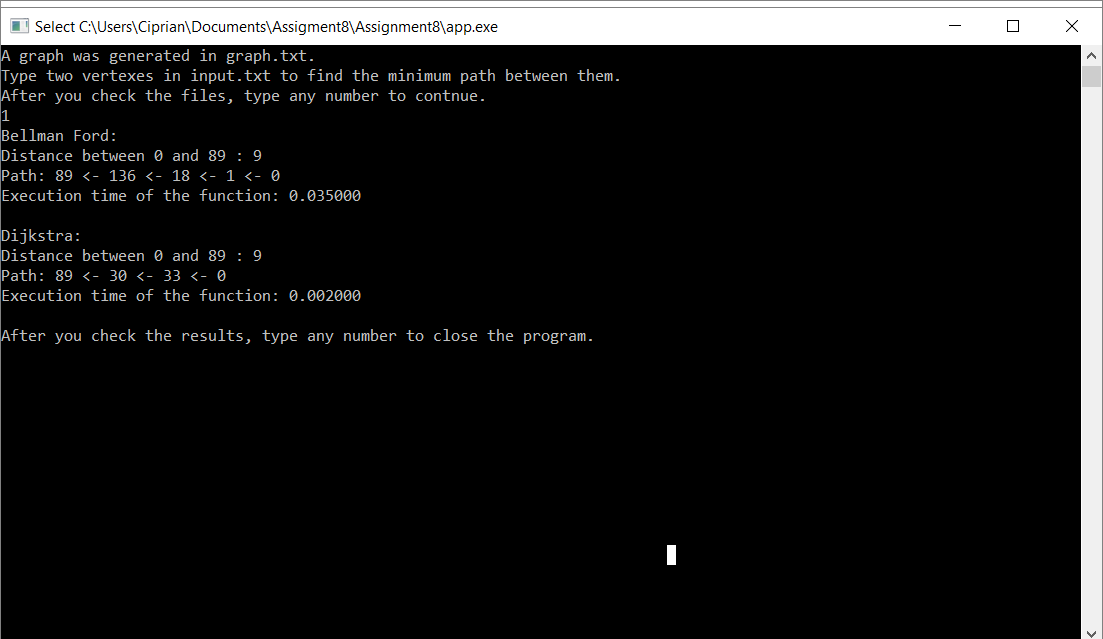
\includegraphics[scale=0.6]{217.png}
\end{center}

For a random generated graph with 269 vertexes:

\begin{center}
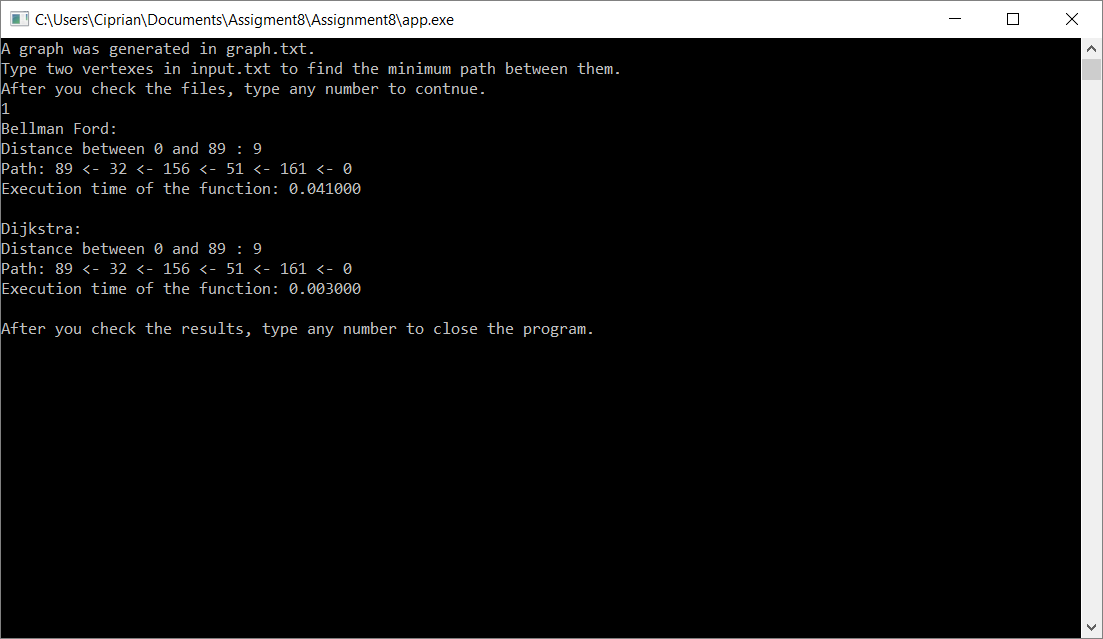
\includegraphics[scale=0.6]{269.png}
\end{center}

For a random generated graph with 341 vertexes:

\begin{center}
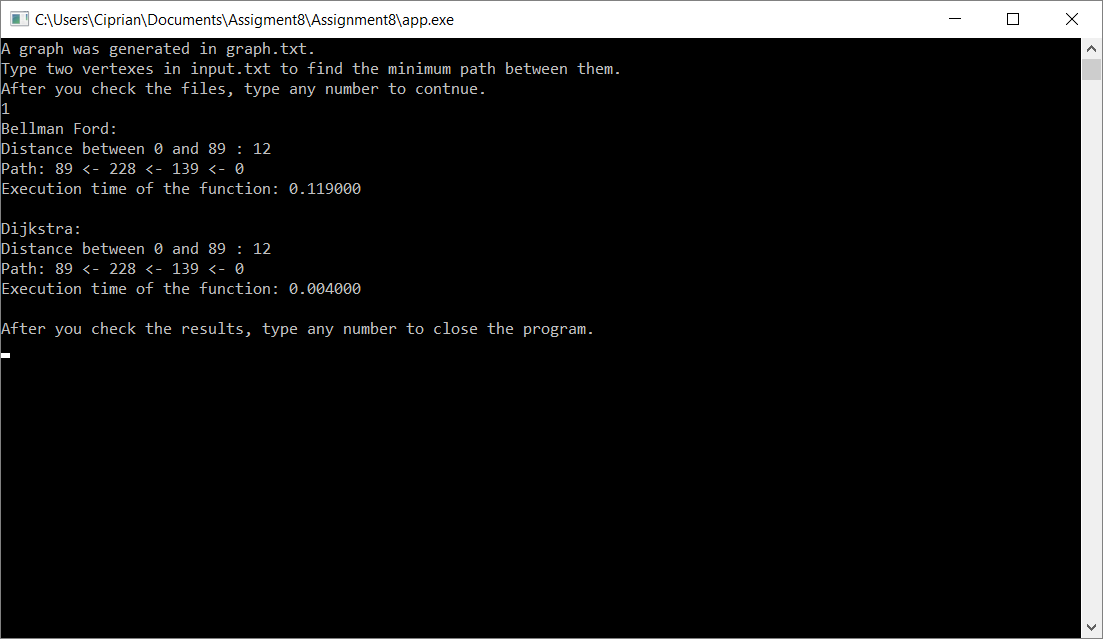
\includegraphics[scale=0.6]{341.png}
\end{center}

For a random generated graph with 478 vertexes:

\begin{center}
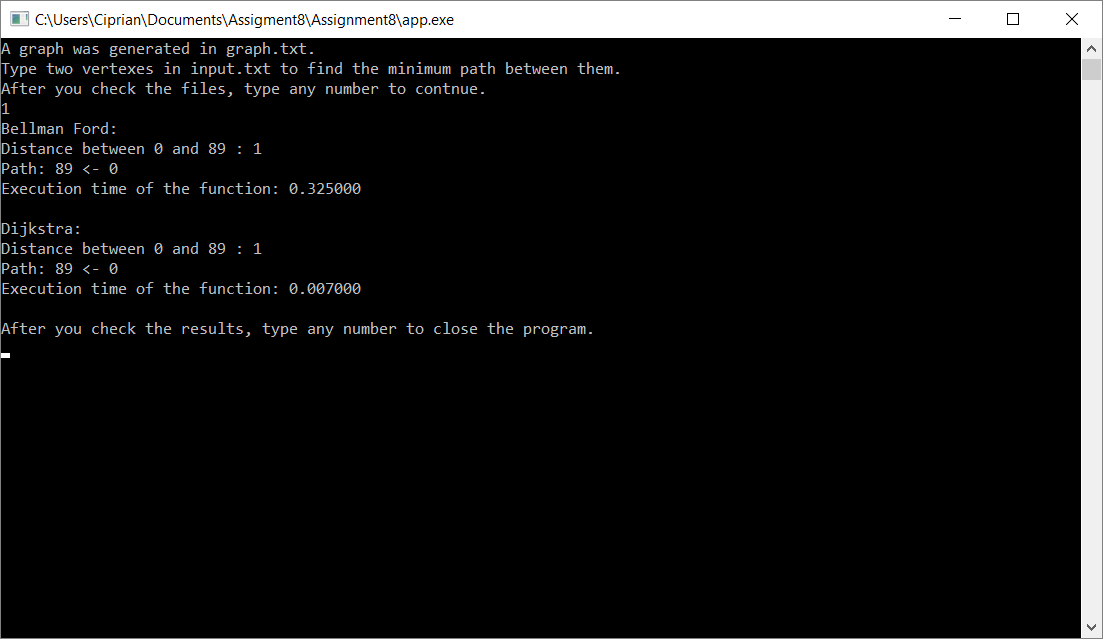
\includegraphics[scale=0.6]{478.png}
\end{center}

From the above pictures and other tests I ran You can observe easily the difference between the execution time of the two algorithms, namely Dijkstra is faster than the Bellman-Ford implementation because Dijkstra implementation has a greedy programming approach and Bellman-Ford implementation is a dynamic approach which offers an optimal solution, but it requires a higher execution time. 

\section{Conclusion}
\textbf{}

After this project I gained a better understanding of the graph theory.

The most challenging part of the assignment was the adapting of the algorithms to store and print the path between the two vertexes. 

I would like to use one on this algorithms in future for a video game with a minimap or an app based in gps locations. Also, I am interested in the implementation of graphs and this algorithms in other programming languages.

\newpage
\section{References}

\textbf{Book}:

Name : Totul despre C si C++ 

Year of publication  :2005

Publisher :Teora

Author :Dr. Kris Jamsa Lars Klander\\
\textbf{Web references}:

$1.http://www.geeksforgeeks.org$

$2. https://www.sharelatex.com/learn/Main_Page$

$3. https://www.thecrazyprogrammer.com$

\end{document}